\documentclass[onecolumn, draftclsnofoot,10pt, compsoc]{IEEEtran}
\usepackage{graphicx}
\usepackage{url}
\usepackage{setspace}
\makeindex
\usepackage{geometry}
\geometry{textheight=9.5in, textwidth=7in}

% 1. Fill in these details
\def \CapstoneTeamName{		Project Chiron}
\def \CapstoneTeamNumber{		4}
\def \GroupMemberOne{			Marie Bomber}
\def \GroupMemberTwo{			Aaron Leondar}
\def \GroupMemberThree{			Hadi Rahal-Arabi}
\def \CapstoneProjectName{			Robotic Wheelchair Data Collection and Analysis}
\def \CapstoneSponsorCompany{	Oregon State University}
\def \CapstoneSponsorPerson{	Matthew William Shuman	}

% 2. Uncomment the appropriate line below so that the document type works
\def \DocType{	%Problem Statement
				Requirements Document
				%Technology Review
				%Design Document
				%Progress Report
				}
\bibliographystyle{ieeetran}	
\newcommand{\NameSigPair}[1]{\par
\makebox[2.75in][r]{#1} \hfil 	\makebox[3.25in]{\makebox[2.25in]{\hrulefill} \hfill		\makebox[.75in]{\hrulefill}}
\par\vspace{-12pt} \textit{\tiny\noindent
\makebox[2.75in]{} \hfil		\makebox[3.25in]{\makebox[2.25in][r]{Signature} \hfill	\makebox[.75in][r]{Date}}}}
% 3. If the document is not to be signed, uncomment the RENEWcommand below
%\renewcommand{\NameSigPair}[1]{#1}

%%%%%%%%%%%%%%%%%%%%%%%%%%%%%%%%%%%%%%%
\begin{document}
\begin{titlepage}
    \pagenumbering{gobble}
    \begin{singlespace}
        \hfill 
        % 4. If you have a logo, use this includegraphics command to put it on the coversheet.
        %\includegraphics[height=4cm]{CompanyLogo}   
        \par\vspace{.2in}
        \centering
        \scshape{
            \huge CS Capstone \DocType \par
            {\large 27 October 2017}\par
            \vspace{.5in}
            \textbf{\Huge\CapstoneProjectName}\par
            \vfill
            {\large Prepared for}\par
            \Huge \CapstoneSponsorCompany\par
            \vspace{5pt}
            {\Large\NameSigPair{\CapstoneSponsorPerson}\par}
            {\large Prepared by }\par
            Group\CapstoneTeamNumber\par
            % 5. comment out the line below this one if you do not wish to name your team
            \CapstoneTeamName\par 
            \vspace{5pt}
            {\Large
                \NameSigPair{\GroupMemberOne}\par
                \NameSigPair{\GroupMemberTwo}\par
                \NameSigPair{\GroupMemberThree}\par
            }
            \vspace{20pt}
                    \begin{abstract}
            	% 6. Fill in your abstract    
  Filler
            \end{abstract} 
        }   
    \end{singlespace}
\end{titlepage}
\newpage
\pagenumbering{arabic}
\tableofcontents
%\listoffigures
%\listoftables
\clearpage

% 8. now you write!
\section{Introduction}
\subsection{Purpose}
This requirements document is intended to define the critical features and functionality of the software interface for Project Chiron. It is intended to act as an agreement between the client Matthew Shuman and the developers, Marie Bomber, Aaron Leondar and Hadi Rahal-Arabi (and any other relevant stakeholders) as to the components of the running and storage of user test data.
\subsection{Scope}
The intent of this project is to produce a Project Chiron interface to be used to collect user test data when navigating a course using a Perimobile wheelchair. This project will not cover the modifications made to a Perimobile wheelchair and will not include any hardware work with the exception of documenting any already-existing hardware modifications. The goal of this project is to create an easy to use interface to begin and record user tests, and allow testing data to be retrieved so a researcher can run POMDP analysis on the gathered results.
\subsection{Definitions, Acronyms and Abbreviations}
This document will use the following definitions:\\
Bag:\\ Collection of data points created by the ROSbag library during a user test\\
Researcher:\\ Admin level user of the Project Chiron Interface. The researcher is expected to have full access to all user testing data (including names)\\
POMDP:\\ Partially Observable Markov Decision Process. This is a mathematical model that can capture the domain dynamics that include uncertainty in action effects and uncertainty in perceptual stimuli. Once a problem is captured as POMDP, it them becomes more ammendable for solution using optimization techniques. \cite{1}
ROS:\\ Robot Operating System\\
Tester:\\ Mid level user of the Project Chiron Interface. The tester is expected to be able to initiate a user test, but will not be able to retrieve all user data. (May be able to retrieve data via an ID, but will not have access to testee names).\\
Testee:\\ Individual who has no access to the Project Chiron interface, but will have a name and ID entry and who will run a user test.\\
User Test:\\ Instance of a single navigation of the testing course. This test will produce a bag of testee data that the Chiron interface must be able to store and retrieve.\\
\subsection{References}
\bibliography{Bibliography}
\section{Overall Description}
\subsection{Wheelchair to Application Communication}
\begin{itemize}
	\item Application must connect with the wireless network of the wheelchair.
	\subitem Receives bags the robot sends after each trial.
	\item The bags, when stored, must contain:
	\subitem The length of time of the trial.
	\subitem The date and time the trial was performed.
	\subitem the ID of the participant.
	\subitem Any relevant sensor information.
	\item Bags cannot contain more than strictly required data because all bags must fit on a moderately-sized flash drive (no more than 16GB).
	\item Bags should not exceed 20MB each.
	\item The bags must be able to be sorted by date/time, and also by the participant's ID.
\end{itemize}
\subsection{Core Architecture}
\subsubsection{Bag and UI interface}
\begin{itemize}
	\item The core system should be able to accept a collected bag and correlate it with input from the user interface to create a data entry.
	\subitem The system should recognize if the user entered is a new testee or previous testee and link the new test to previous information.
	\item When passed a request from the user interface, the core system should pass the query to the main storage medium and return from the query in a format that meets the User Interface needs.
	\item The core system should securely store user logins and accept login requests so the interface only requires to handle pass/no pass scenarios.
\end{itemize}
\subsubsection{Data Storage}
\begin{itemize}
	\item The data entry must be stored in a secure storage space that complies with the Institutional Review Board as defined by the client.
	\subitem Testee names must be separate from a unique ID.
	\subitem The reference link between testee names and ID's must be able to be purged at the client's request.
	\item All user tests (approximately 150 tests) must be able to be stored within an 8GB flash drive.
\end{itemize}
\subsection{User Interface}
\begin{itemize}
	\item The tester should be able to see a list of bags, sortable by trial date/time and name or ID of testee.
	\item The tester should experience little latency (less than 500ms) when sorting bags in the interface.
	\item The tester must have a method of exporting bags, or accessing bags outside of the interface.
	\item The interface must be portable, both capable of running externally on a server, or locally.
	\item It must be simple to replace names associated with bags with UIDs, to maintain data integrity but provide confidentiality to the testers.
	\item The interface must not violate IRB compliance.
	\item The interface will have a presentation layer which provides analytics tools for the bag data [GRANULAR REQUIREMENTS FOR PRESENTATION LAYER TO BE NEGOTIATED WITH CLIENT BEFORE FINAL DRAFT]
\end{itemize}
\subsection{Hardware Documentation}
\begin{itemize}
	\item All Hardware that was not included in the off-the-shelf wheelchair must be documented.
	\item Structure of hardware system documentation must be at a level that an electrical engineer can recreate the system
		\subitem Once documentation is completed, it must meet researcher satisfaction
\end{itemize}
[GRANULAR REQUIREMENTS FOR HARDWARE DOCUMENTATION TO BE DISCUSSED WITH CLIENT BEFORE FINAL DRAFT]
\subsection{Assumptions and Dependencies}
\begin{figure}[h!]
	\centering
	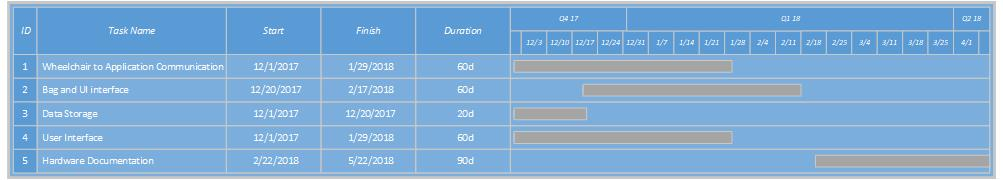
\includegraphics[width=\linewidth, scale=0.7]{PrelimGanttChart.jpg}
\end{figure}

\section{Appendixes}



\end{document}